\documentclass[12pt,a4paper]{article}

% ─── Page Layout ───────────────────────────────────────────────────────────────
\usepackage[a4paper, margin=0.8in, headheight=14pt]{geometry}

% ─── Fonts (XeLaTeX) ───────────────────────────────────────────────────────────
\usepackage{fontspec}
\usepackage{unicode-math}
\setmainfont{TeX Gyre Pagella}
\setmonofont[Scale=0.88]{TeX Gyre Cursor}
\setmathfont{Latin Modern Math}

% ─── Packages ──────────────────────────────────────────────────────────────────
\usepackage{xcolor}
\usepackage{colortbl}
\usepackage{titlesec}
\usepackage{enumitem}
\usepackage{tabularx}
\usepackage{booktabs}
\usepackage{array}
\usepackage{amsmath}
\usepackage{tikz}
\usetikzlibrary{shapes.geometric, arrows.meta, positioning, calc, fit, decorations.pathreplacing}
\usepackage{tcolorbox}
\tcbuselibrary{skins, breakable}
\usepackage{hyperref}
\usepackage{fancyhdr}
\usepackage{graphicx}
\usepackage{microtype}
\hyphenpenalty=10000
\exhyphenpenalty=10000
\sloppy
\usepackage{caption}
\usepackage{setspace}
\usepackage{multirow}
\usepackage{tocloft}

% ─── Q&A helper ────────────────────────────────────────────────────────────────
\newcommand{\Q}[1]{\textbf{#1}\par\noindent\ignorespaces}

% ─── Colour Palette ────────────────────────────────────────────────────────────
\definecolor{myred}{RGB}{196,30,58}
\definecolor{mydark}{RGB}{30,30,50}
\definecolor{mygreen}{RGB}{14,120,80}
\definecolor{myteal}{RGB}{0,130,140}
\definecolor{myamber}{RGB}{180,100,0}
\definecolor{mypurple}{RGB}{100,30,160}
\definecolor{mygray}{RGB}{246,247,249}
\definecolor{mgframe}{RGB}{180,185,200}
\definecolor{watermark}{RGB}{145,150,170}
\definecolor{hdrred}{RGB}{250,232,235}
\definecolor{hdrgreen}{RGB}{220,244,233}
\definecolor{hdrteal}{RGB}{220,242,244}
\definecolor{hdramber}{RGB}{253,242,215}
\definecolor{hdrpurple}{RGB}{238,228,255}
\definecolor{hdrgray}{RGB}{238,240,245}
\definecolor{rowalt}{RGB}{250,251,253}

% ─── Section Formatting ────────────────────────────────────────────────────────
\titleformat{\section}
  {\large\bfseries\color{myred}}{\thesection.}{0.5em}{}
  [\vspace{1pt}{\color{myred}\rule{\linewidth}{0.8pt}}]
\titleformat{\subsection}
  {\normalsize\bfseries\color{myteal}}{\thesubsection}{0.5em}{}
\titlespacing*{\section}{0pt}{18pt}{7pt}
\titlespacing*{\subsection}{0pt}{11pt}{4pt}

% ─── Paragraph ─────────────────────────────────────────────────────────────────
\setlength{\parindent}{0pt}
\setlength{\parskip}{4pt}

% ─── TOC Styling ───────────────────────────────────────────────────────────────
\renewcommand{\cfttoctitlefont}{\large\bfseries\color{myred}}
\renewcommand{\cftaftertoctitle}{\par\noindent{\color{myred}\rule{\linewidth}{0.8pt}}}
\setlength{\cftbeforetoctitleskip}{0pt}
\setlength{\cftaftertoctitleskip}{6pt}
\renewcommand{\cftsecfont}{\normalsize\bfseries\color{mydark}}
\renewcommand{\cftsecpagefont}{\normalsize\bfseries\color{mydark}}
\renewcommand{\cftsecleader}{\cftdotfill{\cftdotsep}}
\setlength{\cftbeforesecskip}{7pt}
\renewcommand{\cftsubsecfont}{\small\color{mydark}}
\renewcommand{\cftsubsecpagefont}{\small\color{mydark}}
\setlength{\cftbeforesubsecskip}{3pt}
\setlength{\cftsubsecindent}{1.4em}

% ─── Table helpers ─────────────────────────────────────────────────────────────
\renewcommand{\arraystretch}{1.45}
\setlength{\tabcolsep}{6pt}
\arrayrulecolor{mydark}
\newcolumntype{B}[1]{>{\small\bfseries\raggedright\arraybackslash}m{#1}}
\newcolumntype{Y}{>{\small\raggedright\arraybackslash}X}
\renewcommand{\tabularxcolumn}[1]{m{#1}}

% ─── Header / Footer ───────────────────────────────────────────────────────────
\pagestyle{fancy}
\fancyhf{}
\fancyhead[L]{\small\color{myred}\textbf{PE-EC603C}\;\color{mydark}--- CMOS VLSI Design}
\fancyhead[R]{\small\color{myteal}\textbf{Module 5 Notes}}
\fancyfoot[C]{\small\color{mydark}\thepage}
\fancyfoot[R]{\small\color{watermark}\textit{\copyright\ Biraj Sarkar}}
\renewcommand{\headrulewidth}{0.5pt}
\renewcommand{\footrulewidth}{0.3pt}

% ─── Hyperref ──────────────────────────────────────────────────────────────────
\hypersetup{
  colorlinks=true, linkcolor=myteal, urlcolor=myteal,
  pdfauthor={Biraj Sarkar},
  pdftitle={PE-EC603C --- Module 5 Notes}
}

% ─── tcolorbox styles ──────────────────────────────────────────────────────────
\tcbset{
  tikzbox/.style={
    colback=mygray, colframe=mgframe, boxrule=0.6pt, arc=4pt,
    left=8pt, right=8pt, top=6pt, bottom=6pt,
    colbacktitle=mgframe, coltitle=mydark,
    fonttitle=\small\bfseries
  },
  defbox/.style={
    colback=hdrgreen, colframe=mygreen, boxrule=0.8pt, arc=4pt,
    left=9pt, right=9pt, top=6pt, bottom=6pt,
    colbacktitle=mygreen, coltitle=white,
    fonttitle=\small\bfseries
  },
  formulabox/.style={
    colback=hdrteal, colframe=myteal, boxrule=0.8pt, arc=4pt,
    left=9pt, right=9pt, top=7pt, bottom=7pt,
    colbacktitle=myteal, coltitle=white,
    fonttitle=\small\bfseries
  },
  examplebox/.style={
    colback=hdramber, colframe=myamber, boxrule=0.8pt, arc=4pt,
    left=9pt, right=9pt, top=6pt, bottom=6pt,
    colbacktitle=myamber, coltitle=white,
    fonttitle=\small\bfseries
  },
  masonbox/.style={
    colback=hdrpurple, colframe=mypurple, boxrule=0.8pt, arc=4pt,
    left=9pt, right=9pt, top=6pt, bottom=6pt,
    colbacktitle=mypurple, coltitle=white,
    fonttitle=\small\bfseries
  },
  exambox/.style={
    colback=hdrpurple, colframe=mypurple, boxrule=1pt, arc=5pt,
    left=10pt, right=10pt, top=8pt, bottom=8pt,
    colbacktitle=mypurple, coltitle=white,
    fonttitle=\bfseries,
    breakable, title after break={\textbf{Frequently Asked / Viva Questions (contd.)}}}
}
% Make all boxes breakable across pages
\tcbset{breakable}

% ─── TikZ styles ───────────────────────────────────────────────────────────────
\tikzset{
  block/.style={rectangle, draw=myteal, fill=hdrteal,
    text width=2.4cm, align=center, minimum height=0.95cm,
    font=\small, rounded corners=3pt, line width=0.7pt},
  redblock/.style={rectangle, draw=myred, fill=hdrred,
    text width=2.4cm, align=center, minimum height=0.95cm,
    font=\small, rounded corners=3pt, line width=0.7pt},
  greenblock/.style={rectangle, draw=mygreen, fill=hdrgreen,
    text width=2.4cm, align=center, minimum height=0.95cm,
    font=\small, rounded corners=3pt, line width=0.7pt},
  amberblock/.style={rectangle, draw=myamber, fill=hdramber,
    text width=2.4cm, align=center, minimum height=0.95cm,
    font=\small, rounded corners=3pt, line width=0.7pt},
  purpblock/.style={rectangle, draw=mypurple, fill=hdrpurple,
    text width=2.4cm, align=center, minimum height=0.95cm,
    font=\small, rounded corners=3pt, line width=0.7pt},
  sumjunc/.style={circle, draw=myamber, fill=hdramber,
    minimum size=0.62cm, font=\small, line width=0.8pt},
  arrow/.style={-Stealth, thick, color=mydark},
  redarrow/.style={-Stealth, thick, color=myred},
  line/.style={thick, color=mydark}
}

% ═══════════════════════════════════════════════════════════════════════════════
\begin{document}
% ═══════════════════════════════════════════════════════════════════════════════

\begin{center}
  {\LARGE\bfseries\color{myred} PE-EC603C --- CMOS VLSI Design}\\[5pt]
  {\normalsize\color{mydark} Semester VI \quad$\bullet$\quad 3L:0T:0P \quad$\bullet$\quad 3 Credits}\\[3pt]
  {\normalsize\color{myteal}\textbf{Module 5 Exam Notes: Dynamic CMOS Circuits \& Sequential Logic}}\\[3pt]
  {\small\color{mydark} CGEC \;$|$\; B.Tech ECE (2023--27) \;$|$\; \textit{Biraj Sarkar}}
\end{center}
\vspace{2pt}
\noindent{\color{myred}\rule{\linewidth}{1.5pt}}
\vspace{2pt}

\hypersetup{linkcolor=mydark}
\tableofcontents
\hypersetup{linkcolor=myteal}
\newpage

% ===============================================================================
\section{CMOS Combinational Logic Gates}
% ===============================================================================

Combinational logic circuits in CMOS are built using complementary networks: a Pull-Up Network (PUN) composed of pMOS transistors and a Pull-Down Network (PDN) composed of nMOS transistors.

\subsection{Static NAND \& NOR Gates}
Static CMOS gates are complementary. For any boolean function, if the nMOS PDN implements the function in its uncomplemented form, the pMOS PUN implements the dual function.

\begin{itemize}[leftmargin=*, itemsep=4pt]
  \item \textbf{2-Input NAND Gate:}
    \begin{itemize}
      \item \textbf{PDN:} Two nMOS transistors connected in series. Both must be ON ($A = B = 1$) to pull the output to GND.
      \item \textbf{PUN:} Two pMOS transistors connected in parallel. If either input is low ($A=0$ or $B=0$), at least one pMOS pulls the output to $V_{DD}$.
      \item \textbf{Sizing:} Since two series nMOS transistors double the pull-down path resistance, each nMOS must be sized $2W_n$ to achieve the same drive current as a standard inverter. The parallel pMOS transistors remain $W_p \approx 2.5W_n$.
    \end{itemize}
  \item \textbf{2-Input NOR Gate:}
    \begin{itemize}
      \item \textbf{PDN:} Two nMOS transistors connected in parallel. If either input is high, the output is pulled to GND.
      \item \textbf{PUN:} Two pMOS transistors connected in series. Both inputs must be low to pull the output to $V_{DD}$.
      \item \textbf{Sizing:} Since two series pMOS transistors double the pull-up path resistance, each pMOS must be sized $2W_p \approx 5W_n$ to match a standard inverter. The parallel nMOS transistors remain $W_n$.
    \end{itemize}
\end{itemize}

\subsection{Complex Logic Gates (AOI \& OAI)}
Complex gates implement multiple logic operations in a single physical gate, reducing transistor count, parasitics, and propagation delay.
\begin{itemize}[leftmargin=*, itemsep=3.5pt]
  \item \textbf{AND-OR-INVERT (AOI):} Implements the function $Y = \overline{(A \cdot B) + C}$.
    \begin{itemize}
      \item \textbf{PDN (AND-OR):} Transistors $A$ and $B$ are in series, and this group is in parallel with transistor $C$.
      \item \textbf{PUN (OR-AND):} Dual network: Transistors $A$ and $B$ are in parallel, and this group is in series with transistor $C$.
    \end{itemize}
  \item \textbf{OR-AND-INVERT (OAI):} Implements the function $Y = \overline{(A + B) \cdot C}$.
    \begin{itemize}
      \item \textbf{PDN (OR-AND):} Transistors $A$ and $B$ are in parallel, and this group is in series with transistor $C$.
      \item \textbf{PUN (AND-OR):} Dual network: Transistors $A$ and $B$ are in series, and this group is in parallel with transistor $C$.
    \end{itemize}
\end{itemize}

% ===============================================================================
\section{Switching \& Transient Characteristics}
% ===============================================================================

The dynamic performance of a digital gate is determined by how quickly it can charge and discharge its output load capacitance.

\subsection{Propagation Delay Derivation ($t_{pHL}, t_{pLH}$)}
Using an equivalent RC model, the propagation delay represents the time taken for the output to reach 50\% of its final value after the input crosses its 50\% value.

Consider a capacitor $C_L$ discharging from $V_{DD}$ to 0 through an nMOS transistor. The transient discharge voltage is governed by the differential equation:
\begin{equation}
  i_D(t) = -C_L \frac{d V_{out}(t)}{d t}
\end{equation}

For a simplified analysis, we approximate the transistor as a constant equivalent resistance $R_{on,n}$ during the transition:
\begin{equation}
  V_{out}(t) = V_{DD} e^{-t / \tau_n} \qquad \text{where} \ \tau_n = R_{on,n} C_L
\end{equation}

To find the high-to-low propagation delay $t_{pHL}$, we solve for $V_{out}(t_{pHL}) = 0.5 V_{DD}$:
\begin{equation}
  0.5 V_{DD} = V_{DD} e^{-t_{pHL} / \tau_n} \implies e^{t_{pHL} / \tau_n} = 2
\end{equation}
\begin{equation}
  t_{pHL} = \ln(2) \tau_n = \ln(2) R_{on,n} C_L \approx 0.69 R_{on,n} C_L
\end{equation}

Similarly, the low-to-high propagation delay $t_{pLH}$ for charging $C_L$ through the pMOS pull-up network is:
\begin{equation}
  t_{pLH} = \ln(2) \tau_p = \ln(2) R_{on,p} C_L \approx 0.69 R_{on,p} C_L
\end{equation}

The average propagation delay $t_p$ of the gate is:
\begin{equation}
  t_p = \frac{t_{pHL} + t_{pLH}}{2}
\end{equation}

\subsection{Rise and Fall Times ($t_r, t_f$)}
\begin{itemize}[leftmargin=*, itemsep=3.5pt]
  \item \textbf{Fall Time ($t_f$):} Time required for the output to drop from 90\% to 10\% of its initial value ($V_{DD}$).
    \begin{equation}
      t_f = t_{10\%} - t_{90\%} = \tau_n \ln(0.1) - \tau_n \ln(0.9) = \tau_n \ln\left(\frac{0.9}{0.1}\right) = \tau_n \ln(9) \approx 2.2 R_{on,n} C_L
    \end{equation}
  \item \textbf{Rise Time ($t_r$):} Time required for the output to rise from 10\% to 90\% of its final value ($V_{DD}$).
    \begin{equation}
      t_r \approx 2.2 R_{on,p} C_L
    \end{equation}
\end{itemize}

\subsection{Parasitic Capacitance Components}
The total load capacitance $C_L$ consists of:
\begin{equation}
  C_L = C_{gate} + C_{diff} + C_{wire}
\end{equation}
\begin{enumerate}[label=\arabic*., leftmargin=*]
  \item \textbf{Gate Capacitance ($C_{gate}$):} The input capacitance of the succeeding logic gates.
  \item \textbf{Diffusion Capacitance ($C_{diff}$):} The drain junction capacitances of the driving gate itself, comprising area and sidewall components: $C_{diff} = A_D C_{j} + P_D C_{jsw}$.
  \item \textbf{Routing/Wire Capacitance ($C_{wire}$):} The capacitance of the metal interconnect lines linking the gates.
\end{enumerate}

% ===============================================================================
\section{Dynamic CMOS Logic Circuits}
% ===============================================================================

Dynamic logic circuits rely on the temporary storage of charge on a high-impedance node rather than continuous static connections.

\subsection{Dynamic Gate Principle and Operation}
A dynamic gate consists of a precharge pMOS ($M_{pre}$), an evaluate nMOS ($M_{eval}$), and an nMOS pull-down logic network (PDN). Its operation is split into two phases controlled by the clock ($\Phi$):

\begin{enumerate}[label=\arabic*., leftmargin=*]
  \item \textbf{Precharge Phase ($\Phi = 0$):}
    \begin{itemize}
      \item $M_{pre}$ is turned ON; $M_{eval}$ is turned OFF.
      \item The path to GND is blocked. The output node charge capacitance $C_L$ charges to $V_{DD}$.
      \item Output = High ('1') regardless of the inputs to the PDN.
    \end{itemize}
  \item \textbf{Evaluation Phase ($\Phi = 1$):}
    \begin{itemize}
      \item $M_{pre}$ is turned OFF; $M_{eval}$ is turned ON.
      \item If the input combination creates a conducting path through the PDN, the output node discharges to GND (Output = '0').
      \item If the PDN is non-conducting, the output node remains at its precharged value $V_{DD}$ via stored charge on $C_L$ (Output = '1').
    \end{itemize}
\end{enumerate}

\subsection{Problems in Dynamic Logic}
Despite having fewer transistors ($N+2$ instead of $2N$) and high speed, dynamic logic suffers from several severe physical issues:

\begin{itemize}[leftmargin=*, itemsep=4pt]
  \item \textbf{Charge Leakage:} During the evaluation phase, if the output node is left floating at $V_{DD}$, leakage currents (subthreshold leakage through the PDN and reverse-biased junction leakage) slowly discharge $C_L$, degrading the logic level. This limits the minimum clock operating frequency.
  \item \textbf{Charge Sharing:}
    If the output is precharged to $V_{DD}$ and an internal node capacitance $C_{int}$ is initially discharged, turning on a subset of the PDN that does not lead to GND will cause the charge on $C_L$ to redistribute with $C_{int}$.
    The final output voltage drops to:
    \begin{equation}
      V_{out} = V_{DD} \left( \frac{C_L}{C_L + C_{int}} \right)
    \end{equation}
    If $V_{out}$ drops below the switching threshold of the next gate, a logic error occurs.
  \item \textbf{Cascading Problem:}
    When dynamic gates are directly cascaded, during precharge, both stage outputs are $V_{DD}$. When evaluation begins ($\Phi = 1$), the inputs to Stage 2 are initially '1'.
    Before Stage 1 can evaluate and drop its output to '0', Stage 2 sees a '1' at its input and begins to discharge its precharged node. Once Stage 2 discharges, it cannot recover since the precharge transistor is OFF. This is a severe race condition.
\end{itemize}

\subsection{Domino Logic}
Domino CMOS logic solves the cascading problem by inserting a static CMOS inverter at the output of every dynamic stage.

\begin{tcolorbox}[defbox, title={\textbf{Domino Logic Mechanism}}]
During precharge ($\Phi = 0$), the dynamic node is charged to $V_{DD}$, making the static inverter output 0. Since the inverter output is 0, the nMOS inputs of all subsequent stages are held OFF. When evaluation begins ($\Phi=1$), the nodes evaluate sequentially like falling dominoes, preventing premature discharge.
\end{tcolorbox}

To prevent charge leakage and charge sharing, a weak pMOS feedback transistor (called a \textbf{keeper}) is added, controlled by the inverter output, to hold the dynamic node at $V_{DD}$ when it is floating.

\begin{tcolorbox}[tikzbox, title={Domino CMOS Logic Gate Circuit Diagram}]
\centering
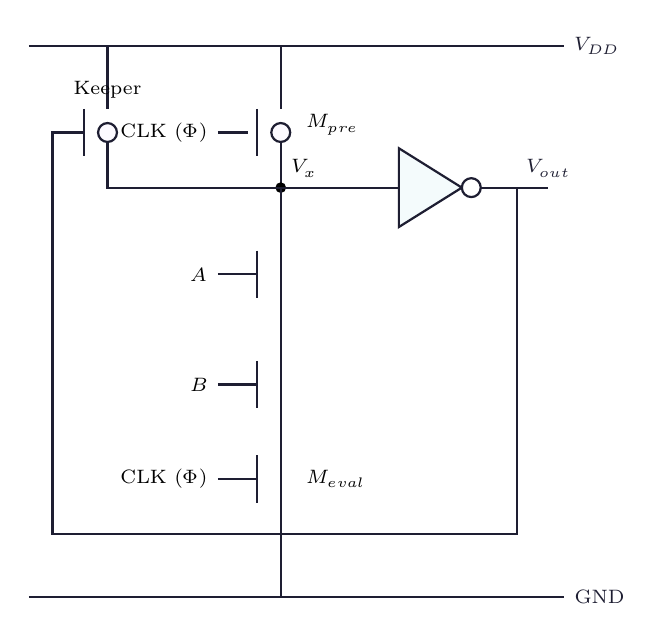
\begin{tikzpicture}[scale=1.0, thick, font=\small]
  % VDD and GND rails
  \draw[line] (-3.2, 4) -- (3.6, 4) node[right, font=\scriptsize] {$V_{DD}$};
  \draw[line] (-3.2, -3) -- (3.6, -3) node[right, font=\scriptsize] {GND};

  % Precharge pMOS (M_pre) at x=0
  \draw[line] (0, 4) -- (0, 3.2);
  \draw[draw=mydark, fill=hdrpurple!20] (0, 2.9) circle (0.12);
  \draw[line] (-0.3, 3.2) -- (-0.3, 2.6); % Gate plate
  \draw[line] (-0.8, 2.9) -- (-0.42, 2.9); % Gate input
  \node[left, font=\scriptsize] at (-0.8, 2.9) {CLK ($\Phi$)};
  \draw[line] (0, 2.78) -- (0, 2.2);
  \node[right, font=\scriptsize] at (0.2, 3.0) {$M_{pre}$};

  % Dynamic Node V_x
  \filldraw (0, 2.2) circle (1.5pt) node[above right, font=\scriptsize] {$V_x$};
  
  % Pull Down Logic Network (PDN) at x=0
  \draw[line] (0, 2.2) -- (0, 1.4);
  % nMOS 1 (Input A)
  \draw[line] (-0.3, 1.4) -- (-0.3, 0.8);
  \draw[line] (-0.8, 1.1) -- (-0.3, 1.1);
  \node[left, font=\scriptsize] at (-0.8, 1.1) {$A$};
  \draw[line] (0, 1.4) -- (0, 0.8);
  
  % nMOS 2 (Input B)
  \draw[line] (0, 0.8) -- (0, 0);
  \draw[line] (-0.3, 0) -- (-0.3, -0.6);
  \draw[line] (-0.8, -0.3) -- (-0.3, -0.3);
  \node[left, font=\scriptsize] at (-0.8, -0.3) {$B$};
  \draw[line] (0, 0) -- (0, -0.6);
  
  % Evaluate nMOS (M_eval) at x=0
  \draw[line] (0, -0.6) -- (0, -1.2);
  \draw[line] (-0.3, -1.2) -- (-0.3, -1.8);
  \draw[line] (-0.8, -1.5) -- (-0.3, -1.5);
  \node[left, font=\scriptsize] at (-0.8, -1.5) {CLK ($\Phi$)};
  \draw[line] (0, -1.2) -- (0, -1.8);
  \draw[line] (0, -1.8) -- (0, -3);
  \node[right, font=\scriptsize] at (0.2, -1.5) {$M_{eval}$};

  % Weak Keeper pMOS (Feedback) at x=-2.2
  \draw[line] (-2.2, 4) -- (-2.2, 3.2);
  \draw[draw=mydark, fill=hdrpurple!20] (-2.2, 2.9) circle (0.12);
  \draw[line] (-2.5, 3.2) -- (-2.5, 2.6); % Gate plate
  \draw[line] (-2.2, 2.78) -- (-2.2, 2.2) -- (0, 2.2); % Drain to Vx
  \node[above, font=\scriptsize] at (-2.2, 3.2) {Keeper};

  % Connection to Static Inverter
  \draw[line] (0, 2.2) -- (1.5, 2.2);
  
  % Inverter Block
  \draw[draw=mydark, fill=hdrteal!30] (1.5, 1.7) -- (2.3, 2.2) -- (1.5, 2.7) -- cycle;
  \draw[draw=mydark, fill=white] (2.42, 2.2) circle (0.12);
  \draw[line] (2.54, 2.2) -- (3.4, 2.2) node[above, font=\scriptsize] {$V_{out}$};

  % Feedback connection from V_out to Keeper gate
  \draw[line] (3.0, 2.2) -- (3.0, -2.2) -- (-2.9, -2.2) -- (-2.9, 2.9) -- (-2.5, 2.9);
\end{tikzpicture}
\end{tcolorbox}

\subsection{NORA Logic}
NORA (No-Race) CMOS logic avoids the static inverter delay of Domino logic by alternating dynamic blocks of opposite logic structures:
\begin{itemize}[leftmargin=*, itemsep=3.5pt]
  \item \textbf{n-tree block:} Uses an nMOS PDN. Precharges to $V_{DD}$ ($\Phi = 0$) and evaluates to GND ($\Phi = 1$).
  \item \textbf{p-tree block:} Uses a pMOS PUN. Precharges to GND ($\Phi = 0$ using an nMOS precharge) and evaluates to $V_{DD}$ ($\Phi = 1$ using a pMOS evaluation transistor).
  \item By cascading an n-tree stage directly into a p-tree stage, the cascading race is eliminated because the outputs are in opposite precharged states.
\end{itemize}

% ===============================================================================
\section{CMOS Sequential Logic Circuits}
% ===============================================================================

Sequential logic circuits use feedback loop topologies to store state.

\subsection{SR Latch}
The SR latch is a bistable circuit. The NAND-based implementation uses cross-coupled NAND gates.
\begin{itemize}[leftmargin=*, itemsep=3pt]
  \item When $S' = 0, R' = 1$, the latch sets ($Q=1, Q'=0$).
  \item When $S' = 1, R' = 0$, the latch resets ($Q=0, Q'=1$).
  \item When $S' = 1, R' = 1$, the latch holds its previous state.
  \item When $S' = 0, R' = 0$, both outputs go to 1 (invalid state).
\end{itemize}

\subsection{D Latch (Transmission Gate Based)}
A D Latch is level-sensitive. It is built using Transmission Gates (TGs) and cross-coupled inverters.
\begin{itemize}[leftmargin=*, itemsep=3.5pt]
  \item A TG consists of an nMOS and a pMOS connected in parallel, controlled by complementary clocks ($CLK$ and $CLK'$). It acts as an ideal bilateral switch with zero voltage degradation.
  \item \textbf{Transparent Mode ($CLK = 1$):} The input TG is ON, passing input $D$ to the output ($Q = D$). The feedback loop is open because the feedback TG is OFF.
  \item \textbf{Hold Mode ($CLK = 0$):} The input TG is OFF, isolating the storage node. The feedback TG is ON, closing the cross-coupled inverter loop to hold the stored state indefinitely.
\end{itemize}

\subsection{D Flip-flop (Master-Slave Configuration)}
An edge-triggered D flip-flop is constructed by cascading two D latches in a Master-Slave structure controlled by complementary clock phases:
\begin{itemize}[leftmargin=*, itemsep=3.5pt]
  \item \textbf{Master Latch:} Level-sensitive, transparent when $CLK=0$, holds when $CLK=1$.
  \item \textbf{Slave Latch:} Level-sensitive, holds when $CLK=0$, transparent when $CLK=1$.
  \item \textbf{Overall Operation:}
    \begin{itemize}
      \item When $CLK = 0$, the Master is transparent (samples input $D$), and the Slave is in hold mode (retains previous state).
      \item On the rising edge of $CLK$ ($0 \to 1$), the Master goes into hold mode, locking the sampled input value. Concurrently, the Slave becomes transparent, passing the locked Master output to the final output $Q$.
      \item This creates a negative-edge or positive-edge triggered behavior depending on clock routing.
    \end{itemize}
\end{itemize}

\newpage
% ===============================================================================
% MANDATORY QUICK REVISION PAGE
% ===============================================================================
\begin{center}
  {\large\bfseries\color{myred} Quick Revision --- Module 5}\\[3pt]
  {\small\color{mydark} Dynamic CMOS Circuits \& Sequential Logic $|$ PE-EC603C}
\end{center}
\noindent{\color{myred}\rule{\linewidth}{1.2pt}}
\vspace{4pt}

\begin{tcolorbox}[formulabox, title={\textbf{Key Equations}}]
$$\text{Propagation Delay:} \quad t_{pHL} \approx 0.69 R_{on,n} C_L \qquad t_{pLH} \approx 0.69 R_{on,p} C_L$$
$$\text{Rise \& Fall Times:} \quad t_f \approx 2.2 R_{on,n} C_L \qquad t_r \approx 2.2 R_{on,p} C_L$$
$$\text{Charge Sharing final voltage:} \quad V_{out,final} = V_{DD} \left( \frac{C_L}{C_L + C_{int}} \right)$$
$$\text{2-Input NAND Sizing:} \quad W_n' = 2W_n, \ W_p' = W_p \qquad \text{2-Input NOR Sizing:} \quad W_n' = W_n, \ W_p' = 2W_p$$
\end{tcolorbox}

\begin{tcolorbox}[defbox, title={\textbf{One-Line Definitions}}]
\begin{itemize}[leftmargin=*, itemsep=2.5pt, topsep=0pt]
  \item \textbf{AOI Gate:} A static CMOS gate implementing series-parallel logic that ANDs, ORs, then inverts the inputs.
  \item \textbf{Propagation Delay:} Average time required for output signal transitions to reach 50\% of their value relative to the input.
  \item \textbf{Dynamic CMOS Logic:} A class of logic gates using clock phases to precharge and evaluate logic on temporary capacitances.
  \item \textbf{Charge Sharing:} Charge redistribution between a floating node and internal node capacitances, causing voltage drops.
  \item \textbf{Domino Logic:} Dynamic CMOS logic configuration with a static inverter at the output to ensure stable cascaded evaluation.
  \item \textbf{Keeper Transistor:} A weak feedback transistor used to combat leakage and noise on dynamic high-impedance nodes.
  \item \textbf{Transmission Gate:} A bilateral analog switch consisting of parallel nMOS and pMOS transistors driven by complementary clocks.
\end{itemize}
\end{tcolorbox}

\begin{tcolorbox}[exambox, title={\textbf{Frequently Asked / Viva Questions}}]
\begin{enumerate}[topsep=0pt, label=\textbf{Q\arabic*.}, itemsep=5pt]
  \item \Q{Why does a series transistor stack require width scaling in static CMOS?}
    In static CMOS, putting transistors in series increases the effective channel length, doubling the resistance for two transistors. To maintain the same drive current (speed) as a standard inverter, the width $W$ of each series transistor must be doubled.
  \item \Q{Derive the propagation delay expression $t_{pHL} = 0.69 R_{on,n} C_L$ using the RC model.}
    For an RC discharge circuit, $V_{out}(t) = V_{DD} e^{-t/RC}$. The propagation delay $t_{pHL}$ is the time when $V_{out}(t_{pHL}) = 0.5 V_{DD} \implies 0.5 V_{DD} = V_{DD} e^{-t_{pHL}/RC} \implies e^{-t_{pHL}/RC} = 1/2 \implies t_{pHL} = RC \ln(2) \approx 0.69 R_{on,n} C_L$.
  \item \Q{What are the primary differences between Rise/Fall time and Propagation Delay?}
    Rise/Fall time ($t_r/t_f$) is the time taken for a single signal to transition between 10\% and 90\% of its peak amplitude. Propagation delay ($t_{pLH}/t_{pHL}$) measures the time difference between the input crossing 50\% and the output crossing 50\% during a transition.
  \item \Q{Explain the precharge and evaluation phases in dynamic CMOS logic.}
    During precharge ($\text{CLK} = 0$), the precharge pMOS is ON, charging the output node to $V_{DD}$, while the evaluate nMOS is OFF. During evaluation ($\text{CLK} = 1$), the precharge pMOS is OFF, the evaluate nMOS is ON, and the output node either discharges to GND or stays high based on the PDN logic state.
  \item \Q{Why cannot raw dynamic CMOS gates be cascaded directly?}
    During precharge, outputs of all stages are high. When evaluation starts, the first stage's output takes a finite time to drop to 0. During this brief interval, the second stage sees a high input and discharges its node prematurely. This discharge is irreversible during that evaluation phase.
  \item \Q{How does Domino CMOS logic solve the cascading problem?}
    Domino logic places a static inverter after the dynamic node. During precharge, the dynamic node is high, making the inverter output 0. Thus, the succeeding stage nMOS inputs are held at 0, preventing them from discharging until the first stage has evaluated and its output transitions.
  \item \Q{What is the function of a keeper transistor in Domino logic?}
    The keeper is a weak pMOS transistor whose gate is driven by the output inverter. When the dynamic node is precharged and remains high, the inverter output is low, turning the keeper ON to pull the node to $V_{DD}$. This counters subthreshold leakage and charge sharing.
  \item \Q{Explain charge sharing in dynamic CMOS and how to mitigate it.}
    Charge sharing occurs when a precharged output node redistributes its charge with internal node capacitances in the PDN when some input switches. It causes the output voltage to drop. Mitigation techniques include adding a keeper transistor or precharging internal nodes to $V_{DD}$ during the precharge phase.
  \item \Q{What is NORA logic and how does it differ from Domino logic?}
    NORA (No-Race) logic alternates n-tree and p-tree dynamic stages rather than using static inverters between stages. The n-tree stages precharge to $V_{DD}$ and evaluate to GND, while the p-tree stages precharge to GND and evaluate to $V_{DD}$, allowing direct cascading.
  \item \Q{Describe the structure and advantage of a Transmission Gate (TG).}
    A TG consists of an nMOS and pMOS in parallel with complementary clock controls. Its main advantage is that it passes a full logic swing (both strong '0' and strong '1') without the threshold voltage drop ($V_{th}$) associated with single-transistor pass logic.
\end{enumerate}
\end{tcolorbox}

\begin{tcolorbox}[tikzbox, title={Static CMOS vs. Dynamic CMOS Logic}]
\renewcommand{\arraystretch}{1.4}
\par\noindent
\begin{tabularx}{\linewidth}{|B{3.2cm}|Y|Y|}
\hline
\textbf{Feature} & \textbf{\color{myred}Static CMOS} & \textbf{\color{myteal}Dynamic CMOS} \\
\hline
\textbf{Transistor Count} & $2N$ transistors (high area). & $N + 2$ transistors (low area). \\
\hline
\textbf{Static Power} & Virtually zero. & Virtually zero. \\
\hline
\textbf{Input Capacitance} & High (gates of both nMOS \& pMOS). & Low (gate of nMOS only). \\
\hline
\textbf{Speed} & Moderate. & High (lower parasitic capacitances). \\
\hline
\textbf{Sensitivity to Noise} & Low (high noise margins). & High (sensitive to leakage \& sharing). \\
\hline
\textbf{Clocking} & No clock required. & Requires a continuous clock signal. \\
\hline
\end{tabularx}
\end{tcolorbox}

\end{document}
